\documentclass[a4paper,12pt,headsepline]{scrartcl}

%\part{title}
\usepackage[utf8]{inputenc}
\usepackage{graphicx}
\usepackage{caption,subcaption}
\usepackage[british]{babel}
\usepackage[T1]{fontenc}
\usepackage{geometry}
\usepackage{proof}
\geometry{left=3.5cm, right=2cm, top=2.5cm, bottom=2cm}
\usepackage{hyperref}
%\usepackage[hyphens,obeyspaces,spaces]{url}
\usepackage{fancybox}
\usepackage{amssymb,amsmath,amsthm}
\usepackage{gensymb}
\usepackage[linesnumbered,ruled,vlined,norelsize]{algorithm2e}
%\usepackage[bookmarksnumbered,pdftitle={\titleDocument},hyperfootnotes=false]{hyperref} 
\usepackage{color}
\usepackage{float}
\usepackage{enumerate}
\usepackage{tikz}
\usetikzlibrary{positioning}

%test
%\usepackage[backend=bibtex]{biblatex}
%\usepackage{filecontents}

%\addbibresource{ref.bib}

\restylefloat{figure}

% Makros
%\newenvironment{sketch}{\begin{proof}[Proof (Sketch)]}{\end{proof}}
%\newtheorem{theorem}{Theorem}
%\newtheorem{assumption}{Assumption}
\newtheorem{lemma}{Lemma}
%\newtheorem{remark}{Remark}
%\newtheorem{definition}{Definition}
%\newtheorem{corollary}{Corollary}
\newcommand{\comment}[1]
{
  \begin{quotation}
    \textcolor{blue}{\underline{Edit:} #1}
  \end{quotation}
}
\newtheorem{aufgabe}{Exercise}
\newcommand{\Ex}[2]
{
	\setcounter{section}{#2}
	\section*{Übungsblatt #2 zu #1}
}
\newcommand{\TODO}[1]
{
  \begin{quotation}
    \textcolor{red}{\underline{TODO:} #1}
  \end{quotation}
}
% Zeichen 
\newcommand{\OO}{\ensuremath{\mathcal{O}}}
\newcommand{\ec}{\texttt{ec}}
\newcommand{\NP}{\call{NP}}
\newcommand{\call}[1]{\ensuremath{\mathcal{#1}}}

% neue Kopfzeilen mit fancypaket
\usepackage{fancyhdr} %Paket laden
\pagestyle{fancy} %eigener Seitenstil
\fancyhf{} %alle Kopf- und Fußzeilenfelder bereinigen
\fancyhead[L]{Benjamin \c Coban \\ Christoph Jabs}
\fancyhead[C]{Algorithmen und Komplexität \\ Blatt 3}
\fancyhead[R]{3526251 \\ 5567177}
\setlength{\headheight}{39pt}
\renewcommand{\headrulewidth}{0.4pt} %obere Trennlinie
%\fancyfoot[C]{\thepage} %Seitennummer
%\renewcommand{\footrulewidth}{0.4pt} %untere Trennlinie

\frenchspacing
\makeindex

% Pseudocode für Java
\usepackage{listings}
\lstset{numbers=left, numberstyle=\tiny, numbersep=5pt, keywordstyle=\color{black}\bfseries, stringstyle=\ttfamily,showstringspaces=false,basicstyle=\footnotesize,captionpos=b}
\lstset{language=java}

% Disable single lines at the start of a paragraph (Schusterjungen)
\clubpenalty = 10000
% Disable single lines at the end of a paragraph (Hurenkinder)
\widowpenalty = 10000
\displaywidowpenalty = 10000

\begin{document}

\begin{aufgabe}
\end{aufgabe}

We can find the specified matching with the help of the following algorithm.
We initialize our new matching $M$ with the intersection of $M_1$ and $M_2$.
To find the remaining edges that should be in $M$, we look at all continuous paths in the symmetic difference between $M_1$ and $M_2$.
For these paths, there are two possibilities, they either have an even length or an odd one.
If a given path has an odd length, we take every second edge in the path (the edges which come from the matching that contributes more edges) and add them to $M$.
If the path has an even length, if the path starts and end in $V_1$, we add all edges in $p$ that are also in $M_1$ to $M$, otherwise we add all the edges which are in $p$ and in $M_2$.

The following pseudocode describes this algorithm more formaly.

\begin{algorithm}[H]
\SetAlgoLined
\KwResult{Find a matching $M$ that matches all the vertices in $V_1$ that are matched by $M_1$ and all the vertices in $V_2$ that are matched by $M_2$}
 $M=M_1\cap M_2$\;
 \ForEach{$p\in$ all continuous paths in $M_1\oplus M_2$}{
  \eIf{$|p|$ is odd}{
    \eIf{$|M_1\cap p|>|M_2\cap p|$}{
      $M=M\cup(M_1\cap p)$\;
    }{
      $M=M\cup(M_2\cap p)$\;
    }
  }{
    \eIf{$p$ starts and ends in $V_1$}{
      $M=M\cup(M_1\cap p)$\;
    }{
      $M=M\cup(M_2\cap p)$\;
    }
  }
 }
 \caption{An algorithm to find the specified matching}
\end{algorithm}

\newpage
\begin{aufgabe}
\end{aufgabe}

\begin{enumerate}[a)]
  \item Consider the following graph:
    \begin{center}
      \begin{tikzpicture}
        [ scale = .75
        , vertex/.style =
          { fill, circle }
        , free/.style =
          { blue }
        , edge/.style =
          { shorten >=2pt, shorten <=2pt, thick }
        , matched/.style =
          { red }
        ]
        \node [vertex,free] (0) {};
        \node [vertex] (1) [above right=.5cm of 0] {};
        \node [vertex] (2) [below right=.5cm of 0] {};
        \node [vertex] (3) [above right=.5cm of 2] {};
        \node [vertex] (4) [below right=.5cm of 2] {};
        \node [] (dots) [below right=.5cm of 4] {\Large$\ddots$};
        \node [vertex] (5) [below right=.5cm of dots] {};
        \node [vertex] (6) [above right=.5cm of 5] {};
        \node [vertex] (7) [below right=.5cm of 5] {};
        \node [vertex,free] (8) [right=.5cm of 7] {};

        \draw [edge] (0) -- (1);
        \draw [edge] (0) -- (2);
        \draw [edge,matched] (1) -- (2);
        \draw [edge] (2) -- (3);
        \draw [edge] (2) -- (4);
        \draw [edge,matched] (3) -- (4);
        \draw [edge] (5) -- (6);
        \draw [edge] (5) -- (7);
        \draw [edge,matched] (6) -- (7);
        \draw [edge] (7) -- (8);
      \end{tikzpicture}
    \end{center}
    If BFS is started from the free vertex on the top left, basically $\frac n3$ and so $\mathcal O(n)$ blossoms need to be shrunken down until the free vertex on the bottom right is reached.

  \item In the algorithm presented in the lecture, the BFS is always restarted from all free vertices of the residual graph $G' =G\setminus B$ if a blossom was found and shrunken. since the path, which was already found until the base of the blossom was reached does not change, the BFS can be continued from the state which it was in when the base of the blossom was reached. The algorithm can be altered in the following way:
\begin{algorithm}[H]
    \SetAlgoLined
    \KwResult{maximal matching $M$ from a general graph $G$}
    $M \gets \emptyset$\\
    \While{$\exists$ augmenting path}{
        Start BFS parallel from all free vertices in $G$\\
        \If{Blossom $B$ found}{
            $G' \gets $ Shrink $B$ to $b$ in $G$\\
            Alter all BFSs which include vertices from $B$ with respect to $b$ so that the new BFS' are semantically equivalent in $G'$ relative to the original BFS in $G$\\
            Continue with the BFS'
        }
        \If{Augmenting path $P$ found}{
                $M \gets M \oplus P$\\
                Unfold $B$ back according to the BFS associated
            }
    }
    
\end{algorithm}

    Runtime:
    \begin{itemize}
        \item one BFS takes $\mathcal{O}(n+m)$
        \item one shrink takes $\mathcal{O}(m)$ therefore BFS $\to$ BFS' takes in $\mathcal{O}(m)$ 
        \item still $\mathcal{O}(n)$ shrinkings in worst case
        \item Between two augmentations the runtime is therefore $\mathcal{O}(n+m)$
        \item Unfolding takes place in $\mathcal{O}(n+m)$ since it is based on the BFS that found the blossom
    \end{itemize}
    In total, one iteration is running in $\mathcal{O}(n+m)$. Since there are up to $\mathcal{O}(n)$ augmentations, the runtime in total is $\mathcal{O}(n\cdot m)$
  
  %However, the path, which was already found until the base of the blossom was reached does not change, so BFS can be continued from the state which it was in when the base of the blossom was reached. 
    %\begin{itemize}
    %  \item BFS (one per augmenting path): $\mathcal O(n+m)$
    %  \item 
    %\end{itemize}
\end{enumerate}

\newpage
\begin{aufgabe}
\end{aufgabe}

Since $G_R$ contains an edge between all tasks that are not connected by a directed path in $D$, an edge $(t_i,t_j)$ in $G_R$ represents that the two tasks $t_i$ and $t_j$ are independent and could therefore be executed in parallel.
A matching in $G_R$ can then be understood as groupings of two tasks that will be scheduled at the same time (i.e. run in parallel on the two machines).

If we consider the maximum matching $M$, then $G_R$ tells us which tasks will run without a ``partner task'' (i.e. the free vertices with respect to $M$) and which tasks are run in parallel with what other task.
Since $M$ is maximum, we can run no more tasks on the second machine, because of the dependencies.
If we look at the runtime, the worst scheduling would have a total runtime of $\tau_\text{worst}^*=|T|$ (no tasks executed in parallel) and for each two tasks we match, we can subtract one unit of time from that.
Therefore the best possible scheduled time is $\tau_\text{best}^*=|T|-|M|$ since $M$ is maximum.
If we consider all schedulings, $\tau^*\ge|T|-|M|$.

\newpage
\begin{aufgabe}
\end{aufgabe}

When starting DFS from vertex 0, we first find the two edges to vertex 1 and then 2.
From there, there are two options how to continue and because vertex 3 has a lower index then vertex 4, we continue in that direction.
We continue with the BFS until we are in the following state:

\begin{center}
  \begin{tikzpicture}
    [ scale = .75
    , vertex/.style =
      { draw, circle }
    , edge/.style =
      { shorten >=2pt, shorten <=2pt, thick }
    , matched/.style =
      { dashed }
    , inpath/.style =
      { blue }
    ]
    \node [vertex,inpath] (0) {0};
    \node [vertex,inpath] (1) [right=.7cm of 0] {1};
    \node [vertex,inpath] (2) [right=.7cm of 1] {2};
    \node [vertex,inpath] (3) [above right=.7cm of 2] {3};
    \node [vertex,inpath] (4) [below right=.7cm of 2] {4};
    \node [vertex,inpath] (5) [right=.7cm of 3] {5};
    \node [vertex,inpath] (6) [right=.7cm of 4] {6};
    \node [vertex] (7) [right=.7cm of 6] {7};
    \node [vertex] (8) [above right=.7cm of 7] {8};
    \node [vertex] (9) [below right=.7cm of 7] {9};
    \node [vertex] (10) [right=.7cm of 8] {10};
    \node [vertex] (11) [below=.7cm of 10] {11};
    \node [vertex] (12) [right=.7cm of 11] {12};

    \draw [edge,inpath,->] (0) -- (1);
    \draw [edge,matched,inpath,->] (1) -- (2);
    \draw [edge,inpath,->] (2) -- (3);
    \draw [edge,inpath,<-] (2) -- (4);
    \draw [edge,matched,inpath,->] (3) -- (5);
    \draw [edge,matched,inpath,<-] (4) -- (6);
    \draw [edge,inpath,->] (5) -- (6);
    \draw [edge] (5) -- (7);
    \draw [edge] (6) -- (7);
    \draw [edge,matched] (7) -- (8);
    \draw [edge] (7) -- (9);
    \draw [edge] (8) -- (9);
    \draw [edge] (8) -- (10);
    \draw [edge] (8) -- (11);
    \draw [edge,matched] (10) -- (11);
    \draw [edge] (11) -- (12);
  \end{tikzpicture}
\end{center}

In this state, we found the blossom containing the vertices 2, 3, 4, 5 and 6 and now need to shrink that blossom into a vertex, which we give the index -1 to:

\begin{center}
  \begin{tikzpicture}
    [ scale = .75
    , vertex/.style =
      { draw, circle }
    , edge/.style =
      { shorten >=2pt, shorten <=2pt, thick }
    , matched/.style =
      { dashed }
    , inpath/.style =
      { blue }
    ]
    \node [vertex] (0) {0};
    \node [vertex] (1) [right=.7cm of 0] {1};
    \node [vertex] (-1) [right=.7cm of 1] {-1};
    \node [vertex] (7) [right=.7cm of -1] {7};
    \node [vertex] (8) [above right=.7cm of 7] {8};
    \node [vertex] (9) [below right=.7cm of 7] {9};
    \node [vertex] (10) [right=.7cm of 8] {10};
    \node [vertex] (11) [below=.7cm of 10] {11};
    \node [vertex] (12) [right=.7cm of 11] {12};

    \draw [edge] (0) -- (1);
    \draw [edge,matched] (1) -- (-1);
    \draw [edge] (-1) -- (7);
    \draw [edge,matched] (7) -- (8);
    \draw [edge] (7) -- (9);
    \draw [edge] (8) -- (9);
    \draw [edge] (8) -- (10);
    \draw [edge] (8) -- (11);
    \draw [edge,matched] (10) -- (11);
    \draw [edge] (11) -- (12);
  \end{tikzpicture}
\end{center}

In this modified graph, we start a new DFS from vertex 0 and get to the following state.

\begin{center}
  \begin{tikzpicture}
    [ scale = .75
    , vertex/.style =
      { draw, circle }
    , edge/.style =
      { shorten >=2pt, shorten <=2pt, thick }
    , matched/.style =
      { dashed }
    , inpath/.style =
      { blue }
    ]
    \node [vertex,inpath] (0) {0};
    \node [vertex,inpath] (1) [right=.7cm of 0] {1};
    \node [vertex,inpath] (-1) [right=.7cm of 1] {-1};
    \node [vertex,inpath] (7) [right=.7cm of -1] {7};
    \node [vertex,inpath] (8) [above right=.7cm of 7] {8};
    \node [vertex,inpath] (9) [below right=.7cm of 7] {9};
    \node [vertex] (10) [right=.7cm of 8] {10};
    \node [vertex] (11) [below=.7cm of 10] {11};
    \node [vertex] (12) [right=.7cm of 11] {12};

    \draw [edge,inpath,->] (0) -- (1);
    \draw [edge,matched,inpath,->] (1) -- (-1);
    \draw [edge,inpath,->] (-1) -- (7);
    \draw [edge,matched,inpath,->] (7) -- (8);
    \draw [edge] (7) -- (9);
    \draw [edge,inpath,->] (8) -- (9);
    \draw [edge] (8) -- (10);
    \draw [edge] (8) -- (11);
    \draw [edge,matched] (10) -- (11);
    \draw [edge] (11) -- (12);
  \end{tikzpicture}
\end{center}

From this state, there is no vertex which we could go to, so we need to backtrack to the last vertex where there is another adjacent edge.
In the given state that is vertex 8.
If we continue from vertex 8 to 10, next we end up in the following state:

\begin{center}
  \begin{tikzpicture}
    [ scale = .75
    , vertex/.style =
      { draw, circle }
    , edge/.style =
      { shorten >=2pt, shorten <=2pt, thick }
    , matched/.style =
      { dashed }
    , inpath/.style =
      { blue }
    ]
    \node [vertex,inpath] (0) {0};
    \node [vertex,inpath] (1) [right=.7cm of 0] {1};
    \node [vertex,inpath] (-1) [right=.7cm of 1] {-1};
    \node [vertex,inpath] (7) [right=.7cm of -1] {7};
    \node [vertex,inpath] (8) [above right=.7cm of 7] {8};
    \node [vertex,inpath] (9) [below right=.7cm of 7] {9};
    \node [vertex,inpath] (10) [right=.7cm of 8] {10};
    \node [vertex,inpath] (11) [below=.7cm of 10] {11};
    \node [vertex] (12) [right=.7cm of 11] {12};

    \draw [edge,inpath,->] (0) -- (1);
    \draw [edge,matched,inpath,->] (1) -- (-1);
    \draw [edge,inpath,->] (-1) -- (7);
    \draw [edge,matched,inpath,->] (7) -- (8);
    \draw [edge] (7) -- (9);
    \draw [edge] (8) -- (9);
    \draw [edge,inpath,->] (8) -- (10);
    \draw [edge,inpath,<-] (8) -- (11);
    \draw [edge,matched,inpath,->] (10) -- (11);
    \draw [edge] (11) -- (12);
  \end{tikzpicture}
\end{center}

Now we found a blossom containing vertices 8, 10 and 11, which we now shrink:

\begin{center}
  \begin{tikzpicture}
    [ scale = .75
    , vertex/.style =
      { draw, circle }
    , edge/.style =
      { shorten >=2pt, shorten <=2pt, thick }
    , matched/.style =
      { dashed }
    , inpath/.style =
      { blue }
    ]
    \node [vertex] (0) {0};
    \node [vertex] (1) [right=.7cm of 0] {1};
    \node [vertex] (-1) [right=.7cm of 1] {-1};
    \node [vertex] (7) [right=.7cm of -1] {7};
    \node [vertex] (-2) [above right=.7cm of 7] {-2};
    \node [vertex] (9) [below right=.7cm of 7] {9};
    \node [vertex] (12) [right=.7cm of -2] {12};

    \draw [edge] (0) -- (1);
    \draw [edge,matched] (1) -- (-1);
    \draw [edge] (-1) -- (7);
    \draw [edge,matched] (7) -- (-2);
    \draw [edge] (7) -- (9);
    \draw [edge] (-2) -- (9);
    \draw [edge] (-2) -- (12);
  \end{tikzpicture}
\end{center}

Now we restart the DFS again and, without the need of backtracking, we find the following augmenting path:

\begin{center}
  \begin{tikzpicture}
    [ scale = .75
    , vertex/.style =
      { draw, circle }
    , edge/.style =
      { shorten >=2pt, shorten <=2pt, thick }
    , matched/.style =
      { dashed }
    , inpath/.style =
      { blue }
    ]
    \node [vertex,inpath] (0) {0};
    \node [vertex,inpath] (1) [right=.7cm of 0] {1};
    \node [vertex,inpath] (-1) [right=.7cm of 1] {-1};
    \node [vertex,inpath] (7) [right=.7cm of -1] {7};
    \node [vertex,inpath] (-2) [above right=.7cm of 7] {-2};
    \node [vertex] (9) [below right=.7cm of 7] {9};
    \node [vertex,inpath] (12) [right=.7cm of -2] {12};

    \draw [edge,inpath,->] (0) -- (1);
    \draw [edge,matched,inpath,->] (1) -- (-1);
    \draw [edge,inpath,->] (-1) -- (7);
    \draw [edge,matched,inpath,->] (7) -- (-2);
    \draw [edge] (7) -- (9);
    \draw [edge] (-2) -- (9);
    \draw [edge,inpath,->] (-2) -- (12);
  \end{tikzpicture}
\end{center}

This is the augmenting path which we wanted to find, but before we can augment the matching, we first need to unfold the shrunken blossoms again:

\begin{center}
  \begin{tikzpicture}
    [ scale = .75
    , vertex/.style =
      { draw, circle }
    , edge/.style =
      { shorten >=2pt, shorten <=2pt, thick }
    , matched/.style =
      { dashed }
    , inpath/.style =
      { blue }
    ]
    \node [vertex,inpath] (0) {0};
    \node [vertex,inpath] (1) [right=.7cm of 0] {1};
    \node [vertex,inpath] (2) [right=.7cm of 1] {2};
    \node [vertex,inpath] (3) [above right=.7cm of 2] {3};
    \node [vertex] (4) [below right=.7cm of 2] {4};
    \node [vertex,inpath] (5) [right=.7cm of 3] {5};
    \node [vertex] (6) [right=.7cm of 4] {6};
    \node [vertex,inpath] (7) [right=.7cm of 6] {7};
    \node [vertex,inpath] (8) [above right=.7cm of 7] {8};
    \node [vertex] (9) [below right=.7cm of 7] {9};
    \node [vertex,inpath] (10) [right=.7cm of 8] {10};
    \node [vertex,inpath] (11) [below=.7cm of 10] {11};
    \node [vertex,inpath] (12) [right=.7cm of 11] {12};

    \draw [edge,inpath,->] (0) -- (1);
    \draw [edge,matched,inpath,->] (1) -- (2);
    \draw [edge,inpath,->] (2) -- (3);
    \draw [edge] (2) -- (4);
    \draw [edge,matched,inpath,->] (3) -- (5);
    \draw [edge,matched] (4) -- (6);
    \draw [edge] (5) -- (6);
    \draw [edge,inpath,->] (5) -- (7);
    \draw [edge] (6) -- (7);
    \draw [edge,matched,inpath,->] (7) -- (8);
    \draw [edge] (7) -- (9);
    \draw [edge] (8) -- (9);
    \draw [edge,inpath,->] (8) -- (10);
    \draw [edge] (8) -- (11);
    \draw [edge,matched,inpath,->] (10) -- (11);
    \draw [edge,inpath,->] (11) -- (12);
  \end{tikzpicture}
\end{center}

And finally, the matching can be augmented:

\begin{center}
  \begin{tikzpicture}
    [ scale = .75
    , vertex/.style =
      { draw, circle }
    , edge/.style =
      { shorten >=2pt, shorten <=2pt, thick }
    , matched/.style =
      { dashed }
    , inpath/.style =
      { blue }
    ]
    \node [vertex] (0) {0};
    \node [vertex] (1) [right=.7cm of 0] {1};
    \node [vertex] (2) [right=.7cm of 1] {2};
    \node [vertex] (3) [above right=.7cm of 2] {3};
    \node [vertex] (4) [below right=.7cm of 2] {4};
    \node [vertex] (5) [right=.7cm of 3] {5};
    \node [vertex] (6) [right=.7cm of 4] {6};
    \node [vertex] (7) [right=.7cm of 6] {7};
    \node [vertex] (8) [above right=.7cm of 7] {8};
    \node [vertex] (9) [below right=.7cm of 7] {9};
    \node [vertex] (10) [right=.7cm of 8] {10};
    \node [vertex] (11) [below=.7cm of 10] {11};
    \node [vertex] (12) [right=.7cm of 11] {12};

    \draw [edge,matched] (0) -- (1);
    \draw [edge] (1) -- (2);
    \draw [edge,matched] (2) -- (3);
    \draw [edge] (2) -- (4);
    \draw [edge] (3) -- (5);
    \draw [edge,matched] (4) -- (6);
    \draw [edge] (5) -- (6);
    \draw [edge,matched] (5) -- (7);
    \draw [edge] (6) -- (7);
    \draw [edge] (7) -- (8);
    \draw [edge] (7) -- (9);
    \draw [edge] (8) -- (9);
    \draw [edge,matched] (8) -- (10);
    \draw [edge] (8) -- (11);
    \draw [edge] (10) -- (11);
    \draw [edge,matched] (11) -- (12);
  \end{tikzpicture}
\end{center}

\end{document}
